% Preamble:
% \usepackage{tikz}

\begin{figure}[ht]
\centering
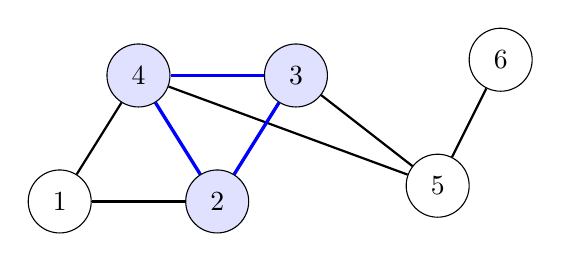
\begin{tikzpicture}[
  v/.style={circle, draw, minimum size=8mm},
  e/.style={thick},
  cliqueV/.style={circle, draw, fill=blue!12, minimum size=8mm},
  cliqueE/.style={very thick, blue}
]

% vertices
\node[v] (1) at (0,0) {1};
\node[cliqueV] (2) at (2,0) {2};
\node[cliqueV] (3) at (3,1.6) {3};
\node[cliqueV] (4) at (1,1.6) {4};
\node[v] (5) at (4.8,0.2) {5};
\node[v] (6) at (5.6,1.8) {6};

% edges (graph)
\draw[e] (1)--(2);
\draw[e] (1)--(4);
\draw[e] (2)--(4);
\draw[e] (2)--(3);
\draw[e] (3)--(4);
\draw[e] (3)--(5);
\draw[e] (5)--(6);
\draw[e] (4)--(5);

% highlight a clique (here: {2,3,4} is a 3-clique)
\draw[cliqueE] (2)--(3);
\draw[cliqueE] (3)--(4);
\draw[cliqueE] (2)--(4);

\end{tikzpicture}
\caption{An example of a clique: vertices $\{2,3,4\}$ form a 3-clique (a $K_3$ subgraph), since every pair among them is connected by an edge.}
\label{fig:clique-example}
\end{figure}
